\chapter{Exports}
\label{export}

When the bricks have been filled and the problem locations are known, it is possible to create picture from schemes. Moreover, those pictures can be highly personalized.
%Une fois les briques remplies et les lieux de problème identifiés, il est possible de générer des images des schémas porteurs d'informations. De plus, il est possible de personnalisé l'apparence de ces schémas pour les adapter au type de diffusion.\\

An export correspond to the personalization of one brick.\\
%Un export correspond à la personnalisation d'un schéma en vue de la génération d'une image.\\


\begin{figure}[h!t]
\centering
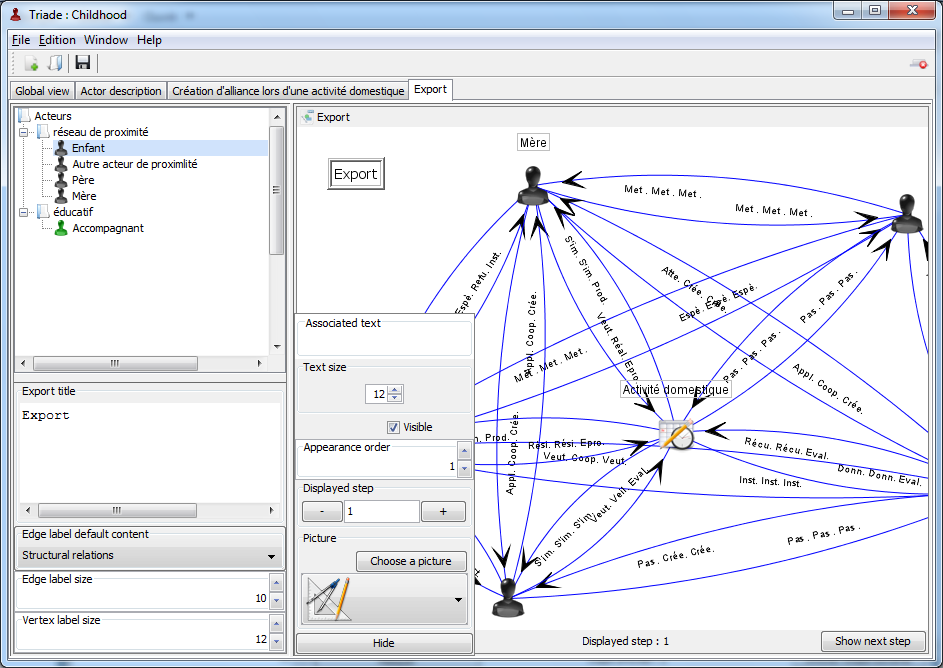
\includegraphics[scale=0.45]{images/vue_export.png}

\caption{An export during its transformation.}

\end{figure}


\section{Creation and access to an export}

There are several way to open an export :\\
%Il existe plusieurs manières de créer un export d'un schéma :\\
\begin{itemize}
\item From a global view, with a right click on one of the bricks. A menu appears with different options, creating a new export of this brick or opening the precedent exports.\\
%\item Depuis une vue globale en faisant un clic droit sur une des briques. Un menu apparaît et permet de créer un nouvel export et d'accéder à tous les export réalisé sur cette brique dans cette session.\\
\item From a brick view, a right click over an empty space in the scheme pop-up the same menu. A right click on an actor allow to open the actor's description. 
%\item Depuis la vue d'une brique, un clic droit sur le schéma au dessus d'aucun sommet fait apparaître le même menu. Un clic droit sur un des sommets permettra d'accéder à la fiche acteur de ce sommet.\\
\item With the folder "exported" in any step folder in the tree on the left of global views.
%\item A l'aide du dossier "exportés" présent dans chaque dossier d'étape dans l'arborescence sur la gauche des vues globales.\\
\end{itemize}

At the begining of export creation, an input field pop-up to define the name of this new export. This name will be displayed in the upper left corner of the generated picture.\\
%Lors de la création d'un export, une boite de dialogue vous invite à saisir le nom qui sera donné à cet export. Il apparaîtra dans un cadre en haut à gauche de l'image générée.\\



\begin{figure}[h!]
\centering
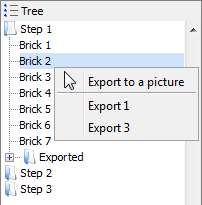
\includegraphics[scale=0.75]{images/menu_export.png}
\caption{The contextual menu to create and access to exports.}
\end{figure}

It is possible to delete an export with a right-click on it in the global view. Once it has been deleted, the export will stay in the list until the next launch of the software.\\

\section{Export aspect personalization}

The appearance of several elements can be transformed in an export :
%De nombreux éléments peuvent être personnalisés dans le cadre d'un export :\\
\begin{itemize}
\item Vertex positions
%\item La position des sommets
\item The label of vertices (actors, meaning or activity) and relations.
%\item Le texte associé à un sommet (acteur, moyen ou activité) ou à une relation.
\item Those text sizes
%\item La taille de ces textes
\item Edge colors
%\item La couleur d'une arête
\item The image of each vertex
%\item L'image utilisée pour représenter un sommet
\item The vertex and edge visibility
%\item La visibilité d'un sommet ou d'une arête
\item The elements apparition order.
%\item L'ordre d'apparition des éléments\\
\end{itemize}
\begin{figure}[h!]
\centering
\subfloat[Of a vertex]{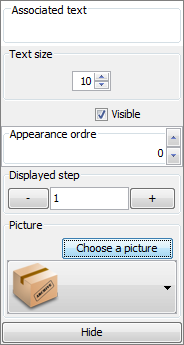
\includegraphics[height=9cm]{images/export_vertex.png}}
\hspace*{35pt}
\subfloat[Of a relation]{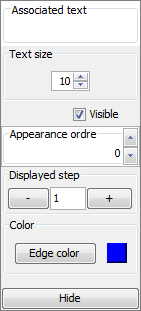
\includegraphics[height=9cm]{images/export_edge.png}}

\caption{The personalization pop-ups}
\label{popup}
\end{figure}

A left click on a vertex or on relation show the associated pop-up.\\
%Il suffit de sélectionner un sommet ou une arête pour faire apparaître le module de personnalisation de cet élément.\\

\subsection{Moving a vertex}
To move a vertex, drag it while pressing "Shift".\\
%Pour déplacer un sommet, il suffit d'appuyer sur la touche "Ctrl" tout en réalisant un clic continu sur le sommet.\\

\subsection{Label editing}
The text field "Associated text" allow the user to define a label for a vertex or a relation. To get the default text, let the field empty. No label will be displayed if there is only a space in the field.\\
%Le champ "Texte associé" permet de modifier l'étiquette d'un sommet ou d'une arête. Pour retrouver le texte initial, il suffit d'effacer complètement le texte saisi. Pour n'afficher aucune étiquette il est possible de ne mettre qu'un espace dans le champ.\\

The label size is controlled by the "Text size" field. The default value is 10.\\
%La modification de la taille du texte d'une étiquette se fait à l'aide du champ "Taille du texte". La valeur par défaut est 10.\\

\subsection{Edge color}
The color of an edge can be selected with the button "Edge color".\\
%Il est possible de choisir la couleur d'une arête avec le bouton correspondant. \\

\subsection{Vertex picture}

It is possible to change the picture of any vertex. The button and the list in the frame "Image" are here for that.\\
%Il est possible de changer les images de chaque sommet. La zone Image contient une liste et un bouton "Choisir une image" à cet effet.\\


The list allow a quick access to all the used pictures. Just click on a picture to associate it to the selected vertex. The button open a window which display all the available pictures.\\ 
%La liste permet d'accéder aux dernières images utilisées. Il suffit de cliquer sur une image pour l'associer au sommet. Le bouton permet d'ouvrir une fenêtre donnant accès à toutes les images disponibles. Sont proposées en premier les images internes à \tria.\\

The check box "Use this image for all the session" will set the selected image for this actor (or meaning or activity) in every export of this session.\\

%Il est possible de cocher la case "Appliquer l'image a toute la session" pour utiliser cette image pour ce sommet dans tous les exports de cette session. Pour annuler ce choix, il suffit de choisir l'image que le sommet avait initialement comme image par défaut.\\ 

\begin{figure}[h!]
\centering
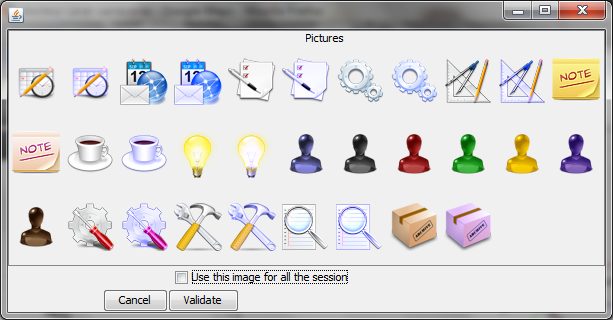
\includegraphics[scale=0.65]{images/choix_image.png}
\caption{The personalized picture window.}
\end{figure}

You can add your own pictures by copying them in the sub-folder "pics" in your \tria installation folder. Those pictures will be automatically resized and the white considered as translucent color. 
% Vous pouvez ajoutez vos propres images en les copiant dans le dossier "Triade/pics" qui se situe dans votre dossier personnel. Ces images seront automatiquement redimensionnée et le blanc sera passé en couleur transparente.\\


\subsection{Element visibilities}
The check box "Visible" allow to hide a vertex or a relation. When a vertex has been hidden, the only way to select it is the tree on the left of the window. To select a hidden relation, drag the window from the first to the second vertex.\\
%La case à cocher "Visible" permet de masquer un sommet ou une arête. Attention, lorsqu'un sommet ou une arête ont été masqués, il n'est plus possible de les sélectionner en cliquant dessus. Il faut passer par l'arborescence sur la gauche pour sélectionner un sommet masqué (un suffixe (caché) est ajouté au nom du sommet). Pour une arête, il faut faire un clic continu à partir du premier jusqu'au deuxième sommet de la relation.\\

If one of the relation extremity is hidden, the relation is not shown. \\
%Les arêtes aboutissant à un sommet masqué ne sont jamais affichées.\\



\subsection{Element apparition order}

In order to make easier the understanding of situation, it is useful to present the different actors of a situation progressively. It's the 
%Afin de présenter plus facilement une situation à des interlocuteurs extérieurs, il peut être utile de faire apparaître progressivement les éléments d'un schéma. L'ordre d'apparition sert à cela.\\

All elements are associated to an apparition order. It is used to determine when an element have to be displayed. For example, a vertex with an apparition order of 2 will be displayed in step 2, 3, ... but not in the first step. 
%Chaque élément (sommet ou arête) est associé à un ordre d'apparition. Il permet déterminer à partir de quand l'élément sera affiché. Par exemple, un sommet ayant un ordre d'apparition à 2 apparaîtra à l'étape 2, 3, etc... mais pas à l'étape 1.\\

The frame "Displayed step" control the current displayed step in the scheme. It is possible to change step with the two buttons in the bottom of the scheme or with the contextual menu.\\
%Le bloc "Etape affichée" permet de contrôler l'étape actuellement affichée dans le schéma. Il est possible de changer l'étape à l'aide des deux boutons situés au dessous du schéma ou à l'aide du menu contextuel qui s'ouvre sur l'ensemble du schéma (clic droit).\\

%Attention, si vous mettez un ordre d'apparition supérieur à l'étape courante, le sommet concerné disparaîtra. Il n'apparaîtra que aux étapes supérieurs à son ordre d'apparition.\\

The step count depend on the greatest apparition order in the scheme. The maximal apparition is 25.\\
%Le nombre d'étape dépend du plus grand ordre d'apparition d'un élément du schéma. L'ordre d'apparition maximal étant 25.\\

Only useful step will be transformed in picture at the end of an export. A step is considered as useful when an element appears during this step.\\
%Lors de la génération de l'image, une image par étape utile sera générée. Une étape utile contient au moins un élément apparaissant à cette étape.\\

\section{Global export settings}
\label{globalExport}
The frame under the actor tree in the left of export window allow to control several settings which affect the whole export.\\
%Le cadre présent sous l'arbre des acteurs sur la gauche de la fenêtre permet de contrôler plusieurs éléments portant sur l'ensemble de l'export.\\

The first field is for editing the title of the export. If this field is let empty, the title will be hidden.\\
%Le premier champ permet de modifier le titre de l'export. Laisser ce champ vide masque le cadre de titre.\\

The next combo control the default edge label. The same possibilities than with the sub-menu "Brick edge labels" are available, but it is also possible to hide all unmodified labels with the "No label" option.\\
%Le champ suivant permet de modifier les étiquettes par défaut des arêtes. Il est possible de masquer l'ensemble des arêtes avec l'option "Aucune étiquette". Cela permet de n'afficher que les étiquettes des arêtes modifiées manuellement.\\

The next two fields control the default size of edge and vertex labels.\\
%Les deux champs suivants permettent de modifier la taille par défaut des étiquettes des sommets et des arêtes.\\

\begin{figure}[h!]
\centering
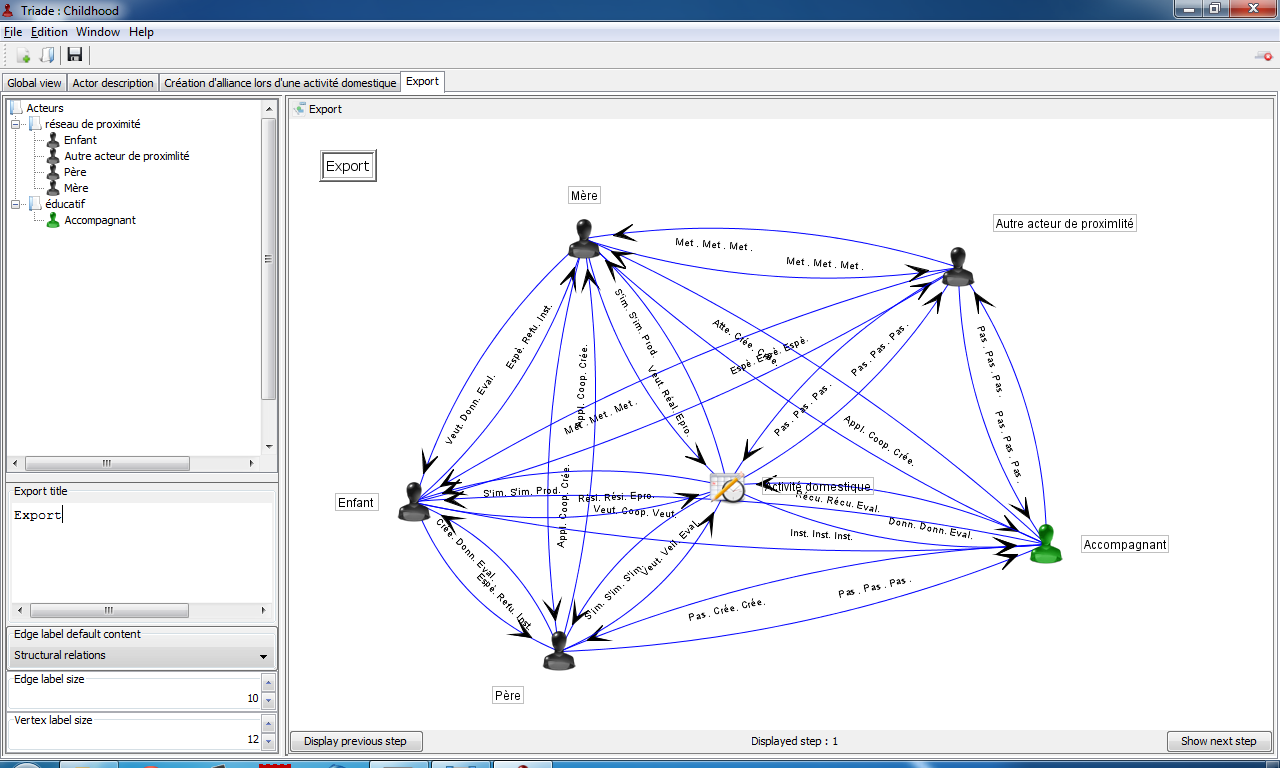
\includegraphics[width=0.5\textwidth]{images/export_global.png}
\caption{The global settings frame is on the bottom left corner.}
\end{figure}

\section{Generate a picture}
When the personalization is finished, it is time to generate the picture(s). A right click on the scheme open a contextual menu with the corresponding option "Generate a picture".\\
%Une fois la personnalisation de l'export terminé, il est nécessaire de générer l'image. Il suffit pour cela de faire un clic droit sur le schéma. La première option du menu contextuel est "Générer une image".\\

A window show to let the user choose where he wants to save the file. If no extension is given, the picture will be a PNG. It is possible to generate JPG, PNG and GIF pictures.\\
%Une fenêtre s'affiche afin de laisser l'utilisateur choisir à quel endroit l'image sera enregistrée. Si aucune extension n'est ajoutée, l'image générée sera au format PNG. Il est cependant possible d'ajouter l'extension de son choix (jpg, png, gif) pour changer de format d'image.\\

If the export contains different apparition order, one picture by useful step will be generated. The name given by the user will be prefixed by "\_Step\_1" for the first step and so.\\
%Si l'export contient plusieurs étapes d'apparition, plusieurs fichiers seront générés. Le nom fourni par l'utlisateur sera préfixé par "\_Etape\_1" pour la première étape et ainsi de suite.\\

\begin{figure}[h!]
\centering
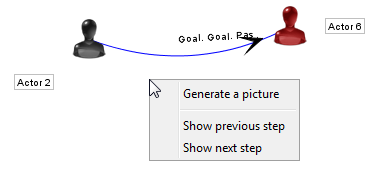
\includegraphics[width=6cm]{images/generer_image.png}

\caption{The picture generation menu}

\end{figure}

  

